\documentclass[journal, spanish]{IEEEtran}

% Paquetes necesarios
\usepackage[T1]{fontenc}
\usepackage[utf8]{inputenc}
\usepackage{babel}
\usepackage{cite}
\usepackage{graphicx}
\usepackage{float}


% Configuración de las cabeceras
\markboth{Diseño de interfaces}{Quiz 3 HTML y CSS}


% Configuración de las secciones
\title{Quiz 3 HTML y CSS}
\author{Alejandra Hernández Bermeo\thanks{} \\
\textit{Fundación Universitaria Konrad Lorenz} \\
}
\begin{document}

% Creación del título
\maketitle


% Introducción
\section{Punto 1}
\begin{center}
  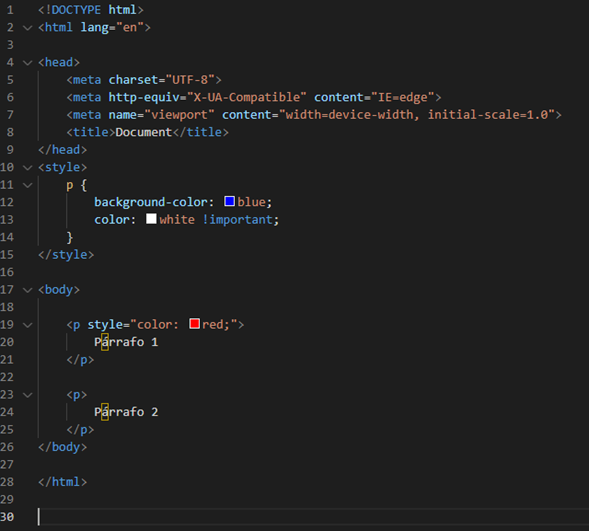
\includegraphics[ height=5cm, width=5cm]{images/1.png}
    \end{center}
Opción correcta:
 b) \begin{center}
  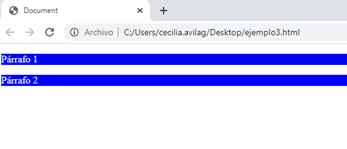
\includegraphics[ height=5cm, width=5cm]{images/4.png}
    \end{center}
- <style>: Este elemento define un bloque de código CSS que define el estilo de los elementos de la página.

- p: Este es el selector CSS que se utiliza para seleccionar todos los elementos <p> de la página.

- background-color: blue;: Este es una propiedad CSS que establece el color de fondo del elemento <p> en azul.

- color: white !important;: Este es otra propiedad CSS que establece el color del texto del elemento <p> en blanco y el !important se utiliza para anular cualquier otro estilo que pueda aplicarse a los elementos <p> en la página.

- <body>: Este elemento marca el inicio del cuerpo de la página, donde se incluyen todos los elementos que se muestran en la página.

- <p style="color:red">: Este es un elemento <p> con un atributo style que define el color del texto en rojo. Aunque se ha definido un estilo en la sección de estilo para todos los elementos <p> en la página, el atributo style en este elemento anula el color de texto definido en el estilo para este elemento en particular.

- <p>: Este es otro elemento <p> que no tiene ningún estilo definido en la página, por lo que usará el estilo definido en la sección de estilo para todos los elementos <p>.


% Resultados
\section{Punto 2}
\begin{center}
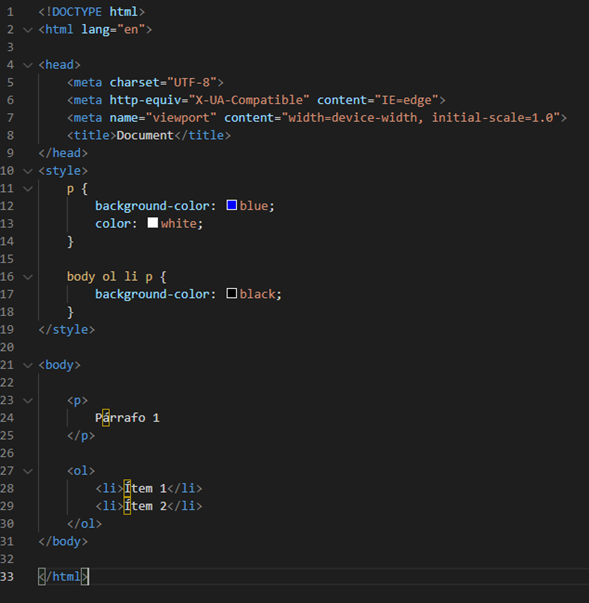
\includegraphics[ height=5cm, width=5cm]{images/2.png}
  \end{center}
Opción correcta:
b) \begin{center}
  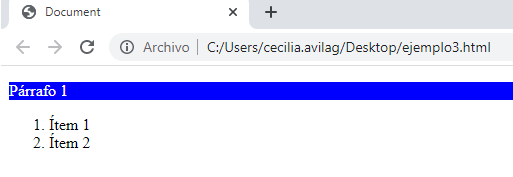
\includegraphics[ height=5cm, width=5cm]{images/5.png}
    \end{center}
- <style>: Este elemento define un bloque de código CSS que define el estilo de los elementos de la página.

- p: Este es el selector CSS que se utiliza para seleccionar todos los elementos <p> de la página.

- background-color: blue;: Este es una propiedad CSS que establece el color de fondo del elemento <p> en azul.

- color: white;: Este es otra propiedad CSS que establece el color del texto del elemento <p> en blanco.

-body ol li p: Este es un selector CSS que se utiliza para seleccionar todos los elementos <p> que se encuentran dentro de un elemento <li> que a su vez está dentro de un elemento <ol> que a su vez está dentro del elemento <body> de la página.

- background-color: black;: Esta es una propiedad CSS que establece el color de fondo del elemento <p> en negro para aquellos que cumplen la regla anterior.

\section{Punto 3}
\begin{center}
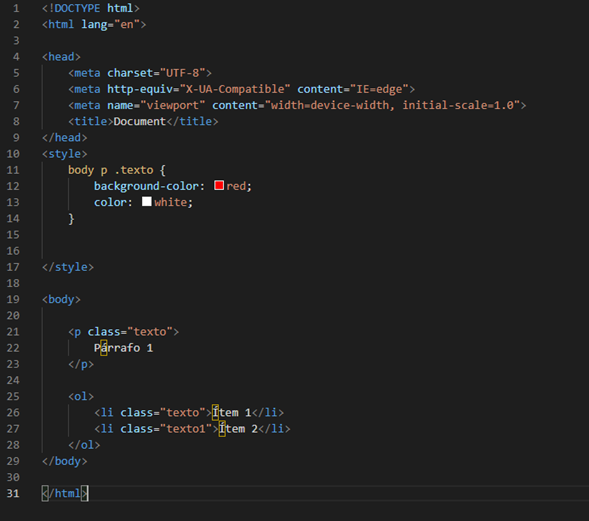
\includegraphics[ height=5cm, width=5cm]{images/3.png}
  \end{center}
Opción correcta:
a) \begin{center}
  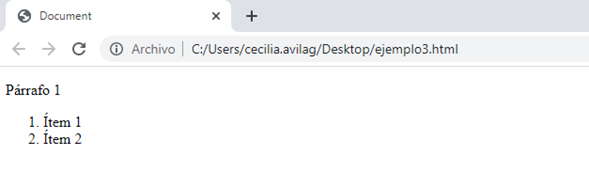
\includegraphics[ height=5cm, width=5cm]{images/6.png}
  \end{center}
  
- <style> es el contenedor para las reglas de estilo CSS.

- body p .texto {background-color: red; color: white;} establece un estilo para el elemento con la clase "texto" dentro de un párrafo dentro del cuerpo del documento. Esto hace que el fondo del texto sea rojo y el color del texto sea blanco.

- <p class="texto"> es un elemento de párrafo con la clase "texto" especificada.

- <ol> es una lista ordenada.

- <li class="texto"> es un elemento de lista con la clase "texto"  especificada.

- <li class="texto1"> es otro elemento de lista con la clase "texto1" especificada (aunque no se define ningún estilo para esta clase en el código), por esto no se pone fondo rojo ni letras blancas

\vspace{12pt}
\end{document}
